\subsection{UC8 – Visualizza informazioni locale}
\begin{center}
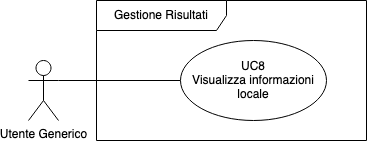
\includegraphics[scale=0.5]{UC_images/UC8.png} 
\end{center}
\begin{itemize}
    \item \textbf{Attore primario}: Utente Generico;
    \item \textbf{Precondizione}: L'utente ha svolto la funzione di ricerca di un locale o sta visualizzando la classifica;
    \item \textbf{Postcondizione}: Vengono visualizzate le informazioni di un locale.
    
    \item \textbf{Scenario principale}: 
    \begin{enumerate}
    \item L'utente seleziona un locale tra quelli presenti nella lista;
    \item Il sistema mostrerà all'utente le informazioni relative al locale scelto.
    \end{enumerate}
\end{itemize}
